%%%%%%%% ICML 2023 EXAMPLE LATEX SUBMISSION FILE %%%%%%%%%%%%%%%%%

\documentclass{article}

% Recommended, but optional, packages for figures and better typesetting:
\usepackage{microtype}
\usepackage{graphicx}
\usepackage{subfigure}
\usepackage{booktabs} % for professional tables

\usepackage{tikz}
% Corporate Design of the University of Tübingen
% Primary Colors
\definecolor{TUred}{RGB}{165,30,55}
\definecolor{TUgold}{RGB}{180,160,105}
\definecolor{TUdark}{RGB}{50,65,75}
\definecolor{TUgray}{RGB}{175,179,183}

% Secondary Colors
\definecolor{TUdarkblue}{RGB}{65,90,140}
\definecolor{TUblue}{RGB}{0,105,170}
\definecolor{TUlightblue}{RGB}{80,170,200}
\definecolor{TUlightgreen}{RGB}{130,185,160}
\definecolor{TUgreen}{RGB}{125,165,75}
\definecolor{TUdarkgreen}{RGB}{50,110,30}
\definecolor{TUocre}{RGB}{200,80,60}
\definecolor{TUviolet}{RGB}{175,110,150}
\definecolor{TUmauve}{RGB}{180,160,150}
\definecolor{TUbeige}{RGB}{215,180,105}
\definecolor{TUorange}{RGB}{210,150,0}
\definecolor{TUbrown}{RGB}{145,105,70}

% hyperref makes hyperlinks in the resulting PDF.
% If your build breaks (sometimes temporarily if a hyperlink spans a page)
% please comment out the following usepackage line and replace
% \usepackage{icml2023} with \usepackage[nohyperref]{icml2023} above.
\usepackage{hyperref}


% Attempt to make hyperref and algorithmic work together better:
\newcommand{\theHalgorithm}{\arabic{algorithm}}

\usepackage[accepted]{icml2023}

% For theorems and such
\usepackage{amsmath}
\usepackage{amssymb}
\usepackage{mathtools}
\usepackage{amsthm}
\usepackage{comment}

% if you use cleveref..
\usepackage[capitalize,noabbrev]{cleveref}

%%%%%%%%%%%%%%%%%%%%%%%%%%%%%%%%
% THEOREMS
%%%%%%%%%%%%%%%%%%%%%%%%%%%%%%%%
\theoremstyle{plain}
\newtheorem{theorem}{Theorem}[section]
\newtheorem{proposition}[theorem]{Proposition}
\newtheorem{lemma}[theorem]{Lemma}
\newtheorem{corollary}[theorem]{Corollary}
\theoremstyle{definition}
\newtheorem{definition}[theorem]{Definition}
\newtheorem{assumption}[theorem]{Assumption}
\theoremstyle{remark}
\newtheorem{remark}[theorem]{Remark}


\newcommand{\pradyumna}[1]{{\color{red}\bf [PM: #1]}}
\newcommand{\swagatam}[1]{{\color{orange}\bf [SH: #1]}}
\newcommand{\gaurav}[1]{{\color{blue}\bf [GN: #1]}}
\newcommand{\farha}[1]{{\color{teal}\bf [FB: #1]}}

% Todonotes is useful during development; simply uncomment the next line
%    and comment out the line below the next line to turn off comments
%\usepackage[disable,textsize=tiny]{todonotes}
\usepackage[textsize=tiny]{todonotes}


% The \icmltitle you define below is probably too long as a header.
% Therefore, a short form for the running title is supplied here:
\icmltitlerunning{Cautious Clicks:\\Analyzing the Perceived Risks on the Web}

\begin{document}

\twocolumn[
% \icmltitle{My Data Literacy Project\\ (Replace this with your Project Title)}

% \icmltitle{Who Hesitates to do What?\\ Analyzing the Perceived Risks on the Web}

\icmltitle{Cautious Clicks:\\Analyzing the Perceived Risks on the Web}



% It is OKAY to include author information, even for blind
% submissions: the style file will automatically remove it for you
% unless you've provided the [accepted] option to the icml2023
% package.

% List of affiliations: The first argument should be a (short)
% identifier you will use later to specify author affiliations
% Academic affiliations should list Department, University, City, Region, Country
% Industry affiliations should list Company, City, Region, Country

% You can specify symbols, otherwise they are numbered in order.
% Ideally, you should not use this facility. Affiliations will be numbered
% in order of appearance and this is the preferred way.
\icmlsetsymbol{equal}{*}

\begin{icmlauthorlist}
\icmlauthor{Farha Baig}{equal,first}
\icmlauthor{Gaurav Niranjan}{equal,second}
\icmlauthor{Pradyumna Yalandur Muralidhar}{equal,third}
\icmlauthor{Swagatam Haldar}{equal,fourth}
\end{icmlauthorlist}

% fill in your matrikelnummer, email address, degree, for each group member
\icmlaffiliation{first}{Matrikelnummer 6639079, farha.baig@student.uni-tuebingen.de, MSc Machine Learning}
\icmlaffiliation{second}{Matrikelnummer 6599177, gaurav.niranjan@student.uni-tuebingen.de, MSc Machine Learning}
\icmlaffiliation{third}{Matrikelnummer 6597371, pradyumna.yalandur-muralidhar@student.uni-tuebingen.de, MSc Machine Learning}
\icmlaffiliation{fourth}{Matrikelnummer 6625573, swagatam.haldar@student.uni-tuebingen.de, MSc Machine Learning}

% You may provide any keywords that you
% find helpful for describing your paper; these are used to populate
% the "keywords" metadata in the PDF but will not be shown in the document
\icmlkeywords{Machine Learning, ICML}

\vskip 0.3in
]

% this must go after the closing bracket ] following \twocolumn[ ...

% This command actually creates the footnote in the first column
% listing the affiliations and the copyright notice.
% The command takes one argument, which is text to display at the start of the footnote.
% The \icmlEqualContribution command is standard text for equal contribution.
% Remove it (just {}) if you do not need this facility.

%\printAffiliationsAndNotice{}  % leave blank if no need to mention equal contribution
\printAffiliationsAndNotice{\icmlEqualContribution} % otherwise use the standard text.

\begin{abstract}
% Put your abstract here. Abstracts typically start with a sentence motivating why the subject is interesting. Then mention the data, methodology or methods you are working with, and describe results.


% Internet and digital media have become an 
% integral part of our daily lives. Various dangers on the web 
% such as data theft, misinformation, public shaming etc. are 
% also on the rise. 
In this report, we study 
the public perception of technology related risks (e.g., fear while expressing opinions on a controversial issue) 
and try to understand the factors that make people sensitive to certain kinds of \emph{risks}. We 
analyse the Internet Supplement from CPS 
Survey and focus on questions on internet usage, concerns, and 
online behaviours which, to the best 
of our knowledge, is previously unexplored. Our contributions include identifying and categorizing features that are deemed important for the risk-perception. The results uncover the interesting insight that over time people are warming up to the convenience of using internet for automated tasks such as banking/shopping, but growing increasingly cautious of social interactions such as sharing opinions. The code and experiments can be found \href{https://github.com/swag2198/data-literacy}{here}.


\end{abstract}

\section{Introduction}\label{sec:intro}

% Motivate the problem, situation or topic you decided to work on. Describe why it matters (is it of societal, economic, scientific value?). Outline the rest of the paper (use references, e.g.~to \Cref{sec:methods}: What kind of data you are working with, how you analyse it, and what kind of conclusion you reached. The point of the introduction is to make the reader want to read the rest of the paper.

% In an era where digital connectivity covers every aspect of our lives, 
The internet has emerged as a powerful tool for communication, information dissemination, and social interaction in this era. However, with the increasing reliance on the online landscape, concerns about privacy, security, and the potential risks associated with internet are also on the rise. This project report studies how the population perceive such technology-induced risks, using a recent ($2021$) dataset from the Current Population Survey (CPS) in the United States (US). The title, ``Cautious Clicks" encapsulates the essence of our research: to unravel the 
%intricacies of 
factors influencing individuals' decisions on a spectrum of things (shown in Figure~\ref{fig:activity-distribution}), 
% from buying goods or services online to posting regular updates on social media and other activities 
on the internet. For the rest of this report, we will keep referring to the activities (that people are often hesitant to do) mentioned in Figure~\ref{fig:activity-distribution}, as ``risks" or ``target variables" interchangeably, and it is for these set of activities that we will analyze the risk-perceptions, which we define as:

\begin{definition}
\label{def:risk-perception}
Given a particular online activity, we define the \emph{risk-perception} associated with it to be the proportion of people who responded in affirmative when asked if they ever hesitated to carry out \emph{that} online activity fearing any kind of privacy or security related concern or social repercussions.
\end{definition}
Risk-perception (for an activity or risk) can also be thought of as the probability that a random person responds positively to such questions. Similarly, the \emph{risk-perception for a group} (e.g., people with income $> 150k$, or with a higher degree) is defined as the same proportion but when the universe of the population is restricted to that group.



% \swagatam{may be the next paragraph goes towards the end of the report}
% \paragraph{Ethical implications} Handling personal data raises privacy concerns. CPS data is anonymized to protect individuals' privacy. It is crucial to tread carefully though, ensuring that our findings are used responsibly and do not inadvertently contribute to discriminatory practices, for example, sensitivity based profiling of individuals and targeted ads. The ethical implications extend to the methodologies and experiments, especially when employing machine learning algorithms to classify and predict internet-related concerns.





% \swagatam{I am putting a rough outline of things to discuss in the introduction, we can expand on them.}

% \begin{itemize}
%     \item public perception of the risks associated with using social media and internet, or the distribution of opinions on internet related threats
%     \item perception of technology related risks falls in 3 broad categories: misinformation, fraud and harrassment --- talk a bit about how our data covers them
%     \item talk about internet usage increasing (cite the blog) and growing crime rates, may be we could also refer to our initial analyses with the us map here)
%     \item why is it important to do this kind of risk-based profiling of the population? Does it have any ethical implications? basically we could expose which demographic variables make people sensitive to certain risks
%     \item 
    
    
% \end{itemize}

\begin{figure}[t]
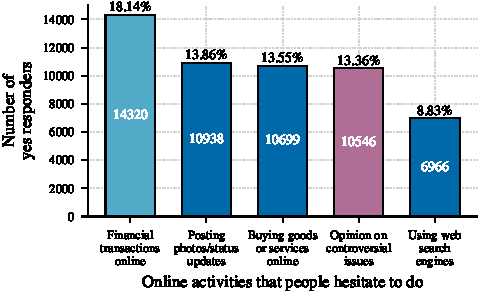
\includegraphics{tex/figures/activity_distribution_2021.pdf}
    \caption{Various online activities and the number of people who expressed their hesitation (risk-perceptions) to do them. Most people ($18.14\%$) have second thoughts while doing \emph{financial transactions}, while $\sim10k$ also expressed unwillingness to do other activities. But \emph{who are these people}, i.e., is there a correlation between other attributes and the tendency to perceive such risks?}
    \label{fig:activity-distribution}
\end{figure}

\paragraph{Outline} 
% \noindent\textbf{Outline:} 
As stated earlier, the aim of this report is to understand which factors shape the risk-perception of the population on digital spaces. We first look at the attribute present in the data: \texttt{HEPSCYBA}, which tells if the respondent has been affected by any kind of cyber crime in real life. We derive the (normalized) cyber crime rate per state using this feature, and plot its geographic distribution over the US states (Fig.~\ref{fig:statewise_distribution}). Interestingly, we also find this distribution correlates  with the internet access/usage rates over the country (Pearson coefficient: $0.46$, $p$-value: $10^{-3}$). To find other factors associated with specific risks, we group the population under different categories and perform hypothesis testing (Sec.~\ref{sec: hyp-test}).
% to test if the groups show varied levels of sensitivity towards a target response (e.g., doing financial transactions).
Sec.~\ref{sec: feat-imp} scales finding correlated features over the large number of features using feature importance scores from an \emph{XGBoost} model.
% However, since our dataset size is quite large with $\sim560$ features, it is difficult to model all such correlated features (and their interactions) by considering all such combinations. Instead, we fit an \emph{XGBoost} predictor on our data, and extract top features using importance scores.
The subsequent importance plots contain a high degree of presence of digital access and wealth related features, which perhaps supports our initial observation of the association between digital access and cyber crime rates over the country. We end this report by looking at how the risk-perceptions evolved (Sec.~\ref{sec: temporal}) over the last four versions of the CPS internet dataset since $2015$.

\begin{figure}[t!]
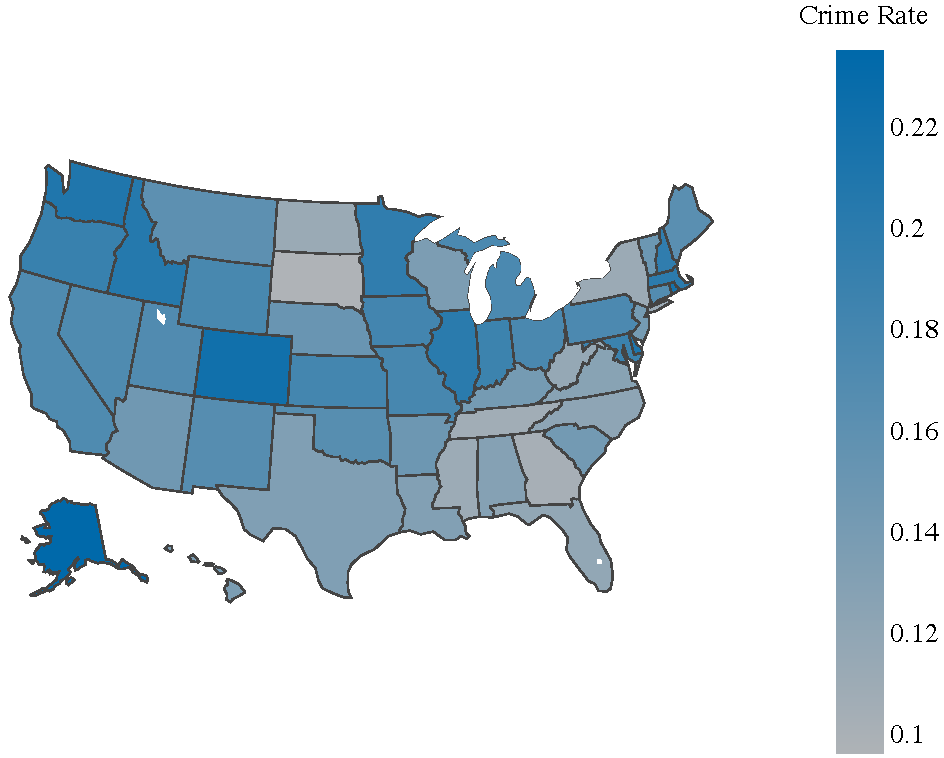
\includegraphics[width=\linewidth]{tex/figures/statewise_distribution.pdf}
\caption{Fraction of people in each US state who were affected by 
% some kind of
online security or data breach, identity theft, or a similar crime on the web. We normalized the total count of affected people by the number of respondents (in each state) to obtain the fractions.}
\label{fig:statewise_distribution}
\end{figure}

\section{Related Works}
This work touches upon several active areas of research in modeling the perception of technology related risks, and understanding fears in digital spaces that we briefly summarize here. ~\citet{knuutila2020global} used the \emph{\href{https://wrp.lrfoundation.org.uk/data-resources/}{2019 World Risk Poll}} dataset to identify three prominent publicly perceived risks on the internet: misinformation, fraud and harrassment. They observed misinformation, i.e., the fear of receiving false information was the most important risk perceived by respondents from over a 100 countries. In a follow-up work~\citep{knuutilaafraid}, they delved deep into the perceived risk of misinformation and found that it varies greatly across geographies.
They also identified that young, educated people worry the most, and degree of actual misinformation and press freedom have little to no correlation with its perceived risk.
None of these works however have considered modeling risk perceptions for other concerns as the world risk poll data had limited information on them.

A recent study~\citep{weeks2024too} analyzed the fears of social judgement or rejection on expressing political opinion on social media. They tried to attribute the fear to the opinion diversity in the respondent's social network, the network's size and various other factors such as sharing or liking political posts, and their political affiliation; and they concluded being embedded in a network with diverse political ideologies actually threatens the individual and decreases the likelihood of expression online. Our work is complementary to this study as we try to identify several other socio-demographic factors correlated with this fear, and we also consider other kinds of seemingly innocuous expressions on social media such as posting photos or texts.

\begin{figure}[t]
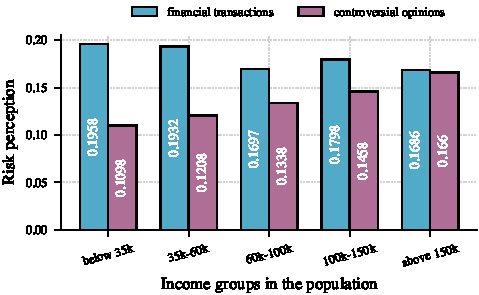
\includegraphics{tex/figures/income_bar_2021.pdf}
    \caption{Here we take two such activities from Figure~\ref{fig:activity-distribution} and see if it correlates with different income groups in the population. We observe that wealthier people tend to become more conservative while expressing opinions on controversial topics online. Interestingly, their concerns on doing financial transactions also drops. More such plots also show similar trends and can be found \href{https://datalitproject1.streamlit.app/}{here}.}
    \label{fig:income-activity-distribution}
\end{figure}


\section{Data}\label{sec:data}

% \paragraph{Data}
We use the \href{https://www.census.gov/data/datasets/time-series/demo/cps/cps-supp_cps-repwgt/cps-computer.html}{Computer and Internet Use Supplement dataset} collected by the US Census Bureau, comprising data collected bi-annually
% at the \pradyumna{individual level}
through a combination of interviews and surveys. This dataset contains responses from over $90k$ individuals, and $\sim560$ attributes that capture several aspects that are of importance to our analysis: job, income, insurance, location, demographics, family, and most importantly, privacy concerns, hesitations, and internet usage. Specifically, the dataset includes yes/no responses to safety-related questions such as \emph{``Have you been affected by an online security breach, identity theft, or a similar crime?"}, and questions relevant to risk-perception such as: \emph{``Have concerns regarding privacy or security stopped you from conducting financial transactions such as banking, investing, or paying bills online?"}. Some example of (coded) raw features in the dataset can be seen in Table~\ref{tab:feature_labelling}.

\section{Methods \& Results}

First, we focus on the latest release of the dataset (November $2021$) to draw some preliminary conclusions, then we also explore data from the previous years (upto $2015$) to analyze overall trends in the risk-perceptions in the digital space, and specifically show how the factors for one particular risk (expressing opinions) evolved during these years.


\subsection{Hypothesis Testing}
\label{sec: hyp-test}
As stated earlier, we treat the online activity related features as response variables and try to find other variables correlated with them. Here we discuss one such example where we try to identify possible correlations between the two reponse variables: hesitates to do financial transactions (lightblue in Fig.~\ref{fig:activity-distribution}), and hesitates to express opinions on controversial issues (violet in Fig.~\ref{fig:activity-distribution}) independently with the annual family income of the respondent. The data has a categorical variable \texttt{HEFAMINC} with 16 levels, ranging from ``less than \$$5k$" to ``\$$150k$ or more". We stratify the population into 5 income groups (x-axis of Fig.~\ref{fig:income-activity-distribution}) following US poverty guidelines for 2021~\cite{poverty_thresholds, poverty_thresholds_yahoo} and assuming average family size of 4 to 6. The response variable on expressing opinions, and the fraction of the people who responded ``yes" to that question seems to show an increasing trend with income as seen in Figure~\ref{fig:income-activity-distribution}.

Here, we want to test if there is some suggestion or evidence of an association between the two variables: the binary response variable, and the explanatory variable income level.
Since both variables are categorical, we consider doing a \emph{chi-square test} to test the null hypothesis that there is no overall difference between people from different income levels with respect to how safe they feel while expressing something controversial on the internet. To perform the test, we first construct the $5\times2$ contingency table (5 income groups, 2 response outcomes) for the two variables, and compute the expected counts under the null hypothesis, that is simply the $($row total $\times$ column total$)$ / total sample size for a $($row, column$)$ cell in the contingency table as also explained in the caption of Table~\ref{tab:contingency_income_response}.

With all the observed and expected counts for the $5\times2$ table, we compute the $\chi^2$ statistic as: $\chi^2 = \sum_{r} \sum_{c} \frac{(O_{rc} - E_{rc})^2}{E_{rc}}$. Since this is two-dimensional table, the degree-of-freedom in our case is $=(R-1)(C-1)=(5-1)(2-1)=4$. The statistic in our case comes out to be $246.37$ with a $p$-value of the order of $10^{-51}$, so we can comfortably reject the null hypothesis, and conclude that there is at least a suggestion of an association between the two variables.




\begin{table}[h]
    \centering
    \begin{tabular}{lcc|r}
\toprule
\textbf{Income levels} & \textbf{Yes} & \textbf{No} & \textbf{Row totals} \\
\midrule
below 35k & $1830$ & $14,844$ & $16,674$ \\
35k-60k & $1948$ & $14,184$ & $16,132$ \\
60k-100k & $2636$ & $17,064$ & $19,700$ \\
100k-150k & $1843$ & $10,796$ & $12,639$ \\
above 150k & $2289$ & $11,499$ & $13,788$ \\
\midrule
\textbf{Column totals} & $10,546$ & $68,387$ & $78,933$ \\
\bottomrule
\end{tabular}
    \caption{Contingency table with observed counts for the income level categorical variable and the binary response variable of hesitation for expressing opinions on controversial topics. Row totals show the sample size of each group. Under null hypothesis, the expected count, for example, for the \emph{below 35k} and the \emph{Yes} entry would be $(16, 674 \times 10,546) / 78,933 \approx 2227.76$.}
    \label{tab:contingency_income_response}
\end{table}


\begin{table}[h]
    \centering
    \begin{tabular}{lll}
\toprule
\textbf{Category} & \textbf{Feature code} & \textbf{Description} \\
\midrule
% Safety& \texttt{HEPSCYBA} & Affected by\\
%                 &&online security\\
%                 &&breach?\\
Digital access & \texttt{HEINTRAV} & 
\begin{tabular}{@{}l@{}}uses internet\\ while travelling? \end{tabular}\\


Online activities & \texttt{HEMEDINF} &
\begin{tabular}{@{}l@{}}gets info. on health\\ or medical topics? \end{tabular}\\


Wealth related & \texttt{PXERN} &
\begin{tabular}{@{}l@{}}weekly overtime\\earnings \end{tabular}\\

% weekly overtime earnings\\
% \begin{tabular}{@{}l@{}}Weekly overtime earnings\end{tabular}\\


% Weekly overtime\\
%                 &&earnings \\

                
% Personal & \texttt{PXNATVTY} & Country of birth \\
% Characteristics\\

\bottomrule
\end{tabular}
    \caption{Features are labelled into $5$ categories for ease of interpretation. In this table, we show one example feature for $3$ categories.}
    \label{tab:feature_labelling}
\end{table}


\subsection{Feature importances using \emph{XGBoost} modeling}
\label{sec: feat-imp}
After analysing the socio-demographic attributes that correlate with 
% privacy concerns and 
hesitations above, we next find other attributes that could affect risk-perceptions on the internet. Since the dataset contains a large number of features, ($\sim560$), we train an \textit{XGBoost} classifier to discover factors relevant for predicting a person's response. Particularly, we use the \textit{XGBoost}~\cite{Chen_2016} model to classify whether an individual is likely to have a privacy related hesitation based on the remaining attributes. We optimize the hyperparameters of the algorithm using the bayesian optimization library~\cite{bayesian_opt}. The model is able to fit to our dataset, with a $3$-fold cross-validation error rate of $\sim8$-$14\%$ for each individual target variable.

Our data contains a large number of fine-grained variables (such as responses to \emph{``Have access to the internet at \textbf{home}?"}, and \emph{``Have access to the internet at \textbf{work}?"}), making it cumbersome to visualize the broad aspects that contribute to risk perception. Hence, we group the top $20$ features into high-level categories as described in Table~\ref{tab:feature_labelling}.

The importance plots\footnote{Please refer to our \href{https://datalitproject1.streamlit.app}{Streamlit web application}.} for several target variables are dominated by aspects that capture digital access and wealth. Figure~\ref{fig:importance_HEPSPRE1} shows important factors for the target variable for risk-perception of financial transactions online. We note that several of the most important features constitute the safety concerns and wealth status of an individual, while we see few attributes related to the mode of access of internet, and no contribution from features belonging to online activities. 

\begin{figure}[t]
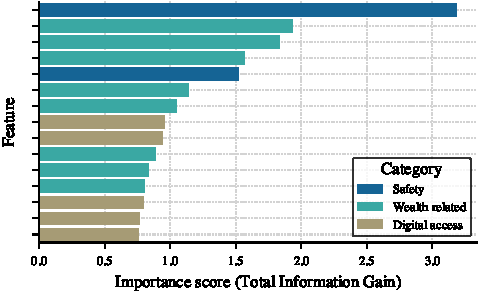
\includegraphics{tex/figures/HEPSPRE1_colored.pdf}
\caption{Top 15 factors by importance for determining the target variable ``hesitates to conduct online financial transactions". We notice three main categories of features: safety, wealth-related, and features that describe modes of digital access, with the latter contributing the least information gain.}

\label{fig:importance_HEPSPRE1}
\end{figure}

\subsection{Evolution of risk-perceptions and their factors}
\label{sec: temporal}
We now study the risk-perception of the online activities over the \emph{years}. Figure~\ref{fig:activity-over-time} shows the trends in the risk perception over the last four surveys, starting from 2015. The risk-perception
% hesitation rate 
for automated financial activities, such as 
conducting bank and e-commerce transactions exhibits 
a steady decline, indicating that people are becoming increasingly comfortable to do them. Further, we notice a steady increase in the hesitation rate for social activities involving other humans, starting from 2017. This prompted us to explore the factors behind hesitation while using social media. We see from Figure~\ref{fig:category_importance_over_time} that online behaviour and wealth related features are rising in significance since 2015, while the means of digital access is losing pertinence.



\begin{figure}[h]
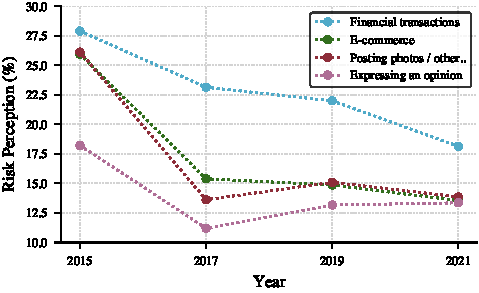
\includegraphics{tex/figures/activity_over_time.pdf}
\caption{Overall trends in hesitation responses from $2015$ to $2021$. We observe that frac. of people fearing to do financial transactions is on a steady decline over the years, however other behavious show non-monotonic trends, e.g., the fear for expressing opinions on controversial topics is actually increasing slowly $2017$ onwards.}
\label{fig:activity-over-time}
\end{figure}



\begin{figure}[h]
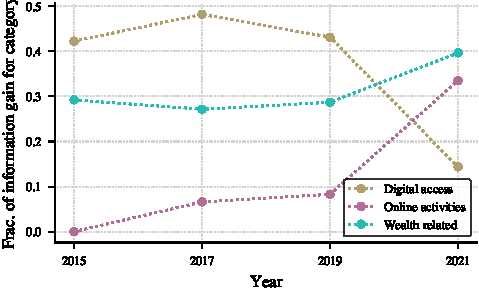
\includegraphics{tex/figures/categories_over_time.pdf}
\caption{Fraction of information gain attributed to the $3$ major categories for the target variable (or risk of) ``expressing opinions online" over the years. The plot shows a steady increase in the fraction of features related to wealth and online behaviour, while the mode of digital access reduces in importance over time.}
\label{fig:category_importance_over_time}
\vspace{-.3cm}
\end{figure}



% \section{Results}\label{sec:results}

% In this section outline your results. At this point, you are just stating the outcome of your analysis. You can highlight important aspects (``we observe a significantly higher value of $x$ over $y$''), but leave interpretation and opinion to the next section. This section absoultely \emph{has} to include at least two figures.


\section{Discussion \& Limitations}\label{sec:conclusion}

We set out to explore factors that affect users' perception of risks while on the internet. To do so, we analysed the US Computer and Internet Use Supplement data. After finding strong correlations with several common socio-demographic variables such as age, education and income levels, we explored other features that are of relevance by ranking them using information gain in a classifier, and found modes of digital access, and wealth related attributes to be major factors. We then looked at trends in risk perception over the last four releases of the dataset, extending upto 2015, which indicated that users are growing increasingly comfortable with the use of technology for automated tasks like finance, while also becoming wary of social interactions such as posting opinions or photos online. 

We acknowledge that the factors we identified from the data might not reflect the true causal relationships in play here, and formulating a qualitative social study trying to understand what caused an individual to have certain fears (e.g., news or personal tragedy) could be a future work.

% Use this section to briefly summarize the entire text. Highlight limitations and problems, but also make clear statements where they are possible and supported by the analysis. 

\section*{Contribution Statement}

Gaurav Niranjan found and preprocessed the datasets and built the webapp. Swagatam Haldar performed the analyses for hypothesis testing. Pradyumna YM led the \emph{XGBoost} importance analysis. Farha Baig produced interactive visualizations on the app. All authors contributed  in annotating the features, making figures and writing this manuscript.
% Explain here, in one sentence per person, what each group member contributed. For example, you could write: Max Mustermann collected and prepared data. Gabi Musterfrau and John Doe performed the data analysis. Jane Doe produced visualizations. All authors will jointly wrote the text of the report. Note that you, as a group, a collectively responsible for the report. Your contributions should be roughly equal in amount and difficulty.

% \section*{Notes} 

% Your entire report has a \textbf{hard page limit of 4 pages} excluding references. (I.e. any pages beyond page 4 must only contain references). Appendices are \emph{not} possible. But you can put additional material, like interactive visualizations or videos, on a githunb repo (use \href{https://github.com/pnkraemer/tueplots}{links} in your pdf to refer to them). Each report has to contain \textbf{at least three plots or visualizations}, and \textbf{cite at least two references}. More details about how to prepare the report, inclucing how to produce plots, cite correctly, and how to ideally structure your github repo, will be discussed in the lecture, where a rubric for the evaluation will also be provided.

\clearpage
\bibliography{bibliography}
\bibliographystyle{icml2023}

\end{document}


% This document was modified from the file originally made available by
% Pat Langley and Andrea Danyluk for ICML-2K. This version was created
% by Iain Murray in 2018, and modified by Alexandre Bouchard in
% 2019 and 2021 and by Csaba Szepesvari, Gang Niu and Sivan Sabato in 2022.
% Modified again in 2023 by Sivan Sabato and Jonathan Scarlett.
% Previous contributors include Dan Roy, Lise Getoor and Tobias
% Scheffer, which was slightly modified from the 2010 version by
% Thorsten Joachims & Johannes Fuernkranz, slightly modified from the
% 2009 version by Kiri Wagstaff and Sam Roweis's 2008 version, which is
% slightly modified from Prasad Tadepalli's 2007 version which is a
% lightly changed version of the previous year's version by Andrew
% Moore, which was in turn edited from those of Kristian Kersting and
% Codrina Lauth. Alex Smola contributed to the algorithmic style files.
